\documentclass{article}
\usepackage{amsmath, amsthm, amssymb, amsfonts, bm}
\usepackage{graphicx}
\usepackage[T1]{fontenc}
\usepackage[utf8]{inputenc}
\usepackage[a4paper]{geometry}
\usepackage{fancyhdr}
\usepackage[algo2e]{algorithm2e}
\fontfamily{cmr}

\title{DD2424 - Assignment 2 (Bonus)}
\author{Oskar Stigland \\ stigland@kth.se}

\pagestyle{fancy}
\fancyhf{}
\rhead{stigland@kth.se}
\lhead{DD2424 - Deep Learning in Data Science}
\rfoot{Page \thepage}

\begin{document}
%\maketitle

	\begin{titlepage}
		\begin{center} 
			
			\rule{\linewidth}{0.5mm}\\[0.5 cm]
			{ \huge \bfseries DD2424 - Assignment 2 (Bonus)}\\[0.3 cm] % Title of your document
			\rule{\linewidth}{0.5mm}\\[1 cm]
					
			\small\vfill
			\begin{center}
			\centering
			{\large \bfseries \textsc{Summary}}\\
			\vspace{1cm}
			\begin{minipage}{10cm}
				
				I have completed both of the bonus problems. For the first part, I have implemented a wider network, i.e. employing more hidden nodes, used dropout, experimented with data augmentation (using both image flipping and translations), as well as implementing an Adam optimizer (rather than Nesterov Momentum). For the second part, I attempted to do some semi-extensive testing, using data augmentation and varying the number of hidden nodes, the regularization parameter and the dropout rate. After the semi-extensive testing, I trained the network for a larger number of steps with the top-performing parameter setting, which yielded a testing accuracy of $\sim 56$\%.
			\end{minipage}
			\end{center}
			\large\vfill
						

		\end{center}	
		
		\begin{minipage}{0.4\textwidth}
			\begin{flushleft} \large
				%\emph{Student:}\\
				Oskar \textsc{Stigland}\\
				DD2424\\
				Spring 2023
			\end{flushleft}
		\end{minipage}	

	\end{titlepage}

\newpage

\section*{Part I}

	To bump up the performance of the network, I attempted to implement a number of the suggested training features. Specifically, I tried to employ a wider network with dropout trained on the full dataset with data augmentation. I tested a number of settings for the width of the network and the dropout rate. It seems that a high dropout rate and a large number of hidden nodes has a declining marginal rate of improvement in terms of the accuracy - perhaps even strictly declining after some threshold. Even when using image flipping and translations, I had a hard time getting more than modest improvements over the $2$-layer network with $50$ hidden nodes trained with a cyclical learning rate and $0 < \lambda < 10^{-3}$.\\\\
%
	I tested the performance of the network for $\lambda \in \{0.0001, 0.0002, 0.00025, 0.0003\}$, using a cyclical learning rate for $3$ cycles, where $\eta_{\text{min}} = 10^{-5}$ and $\eta_{\text{max}} = 10^{-1}$. Then, I also used image flipping and random image translations, where I translated the image with $\bm{x}_{horizontal}, \bm{x}_{vertical}\,\sim Uniform(-3, 3)$. Each image was flipped with $p_{flip} = 0.2$ and translated with $p_{translate} = 0.05$. The network used $100$ nodes in the hidden layer, instead of the original $50$, combined with a dropout rate of $0.2$. The results for the specified lambdas are summarized in the table below. The figures are presented together in Figure $1$, along with the loss and accuracy plots for the top-performing parameter settings. The best performance in terms of testing accuracy was given by $\lambda = 0.00025$ with an accuracy of $53.46$\% - which is a somewhat modest improvement over the smaller $2$-layer network without dropout and data augmentation.
	\vspace{0.3cm}
	\begin{center}	
	\begin{tabular}{|l|c|}
		\hline
		 $\lambda$ & \text{Accuracy}, \% \\ \hline
		0.0001 & 52.98\\ 
		0.0002 & 53.33\\
		0.00025 & 53.46\\
		0.0003 & 53.28\\\hline
	\end{tabular}
	\end{center}

	\begin{figure}[!h]
	\centering
	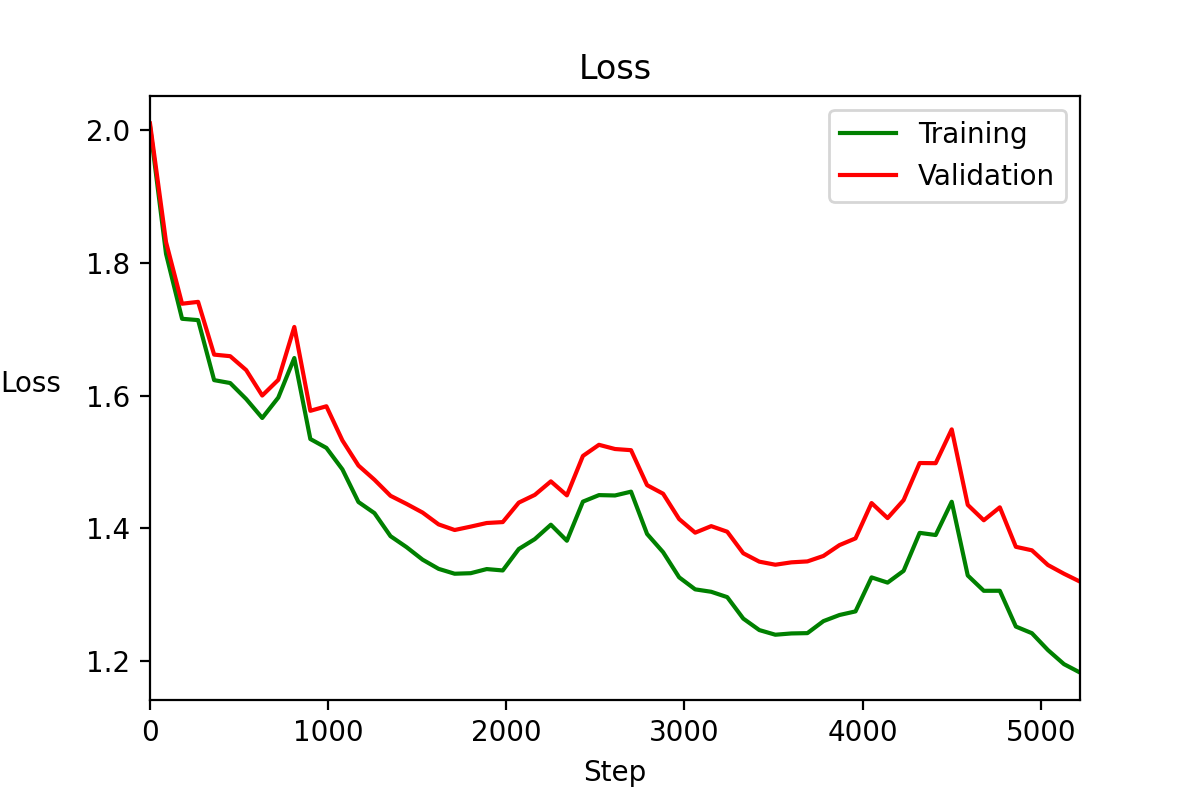
\includegraphics[width=6cm]{../plots/cyclical/loss_v2.png}
	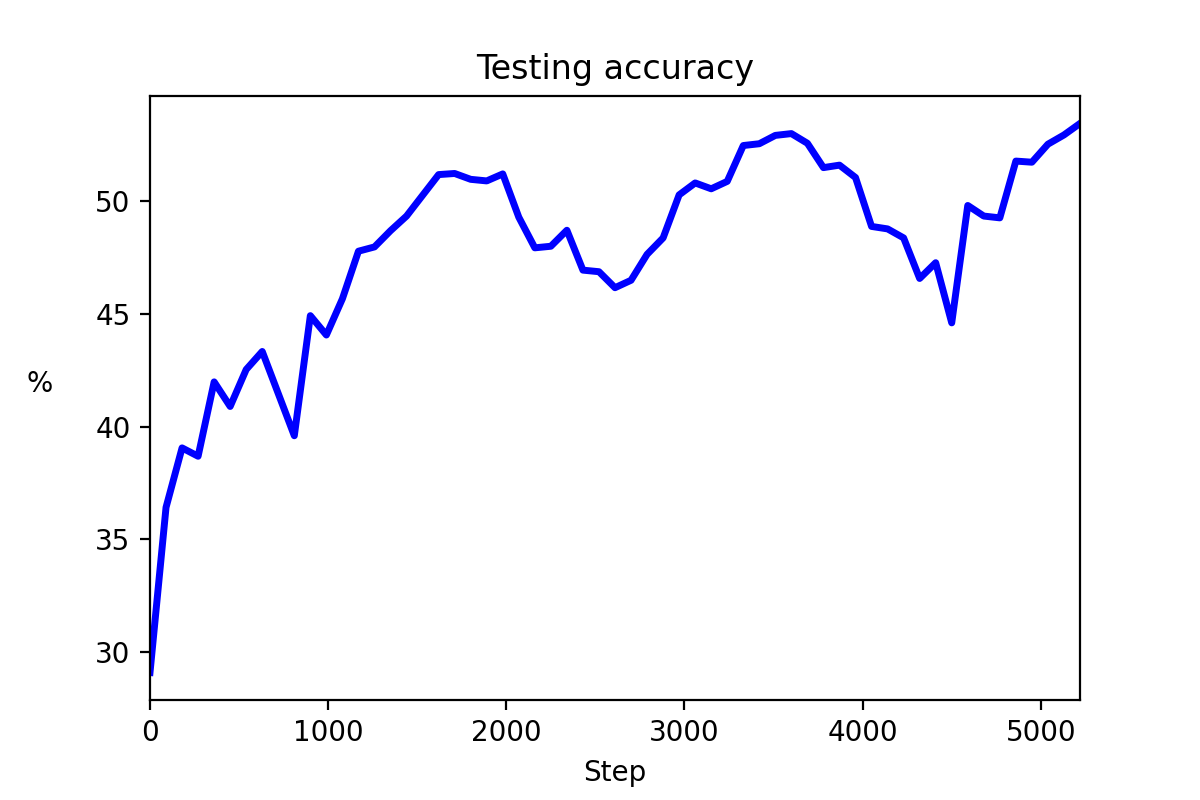
\includegraphics[width=6cm]{../plots/cyclical/acc_v2.png}
	\caption{Loss and testing accuracy when using $m=100$ with a $0.2$ dropout rate, image flipping, image translations and a cyclical learning rate - for $\lambda=0.00025$}
	\end{figure}

%\newpage
%	\begin{figure}[!h]
%		\centering
%		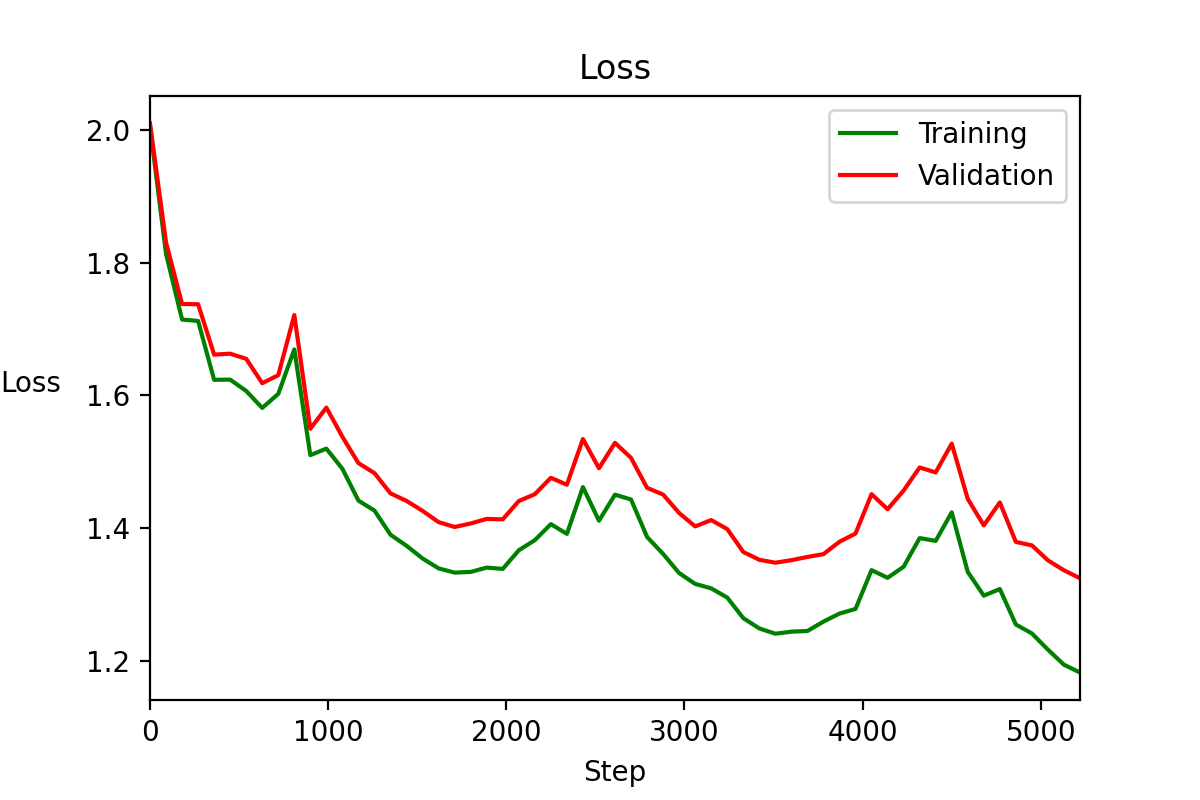
\includegraphics[width=6cm]{../plots/cyclical/loss_v0.png}
%		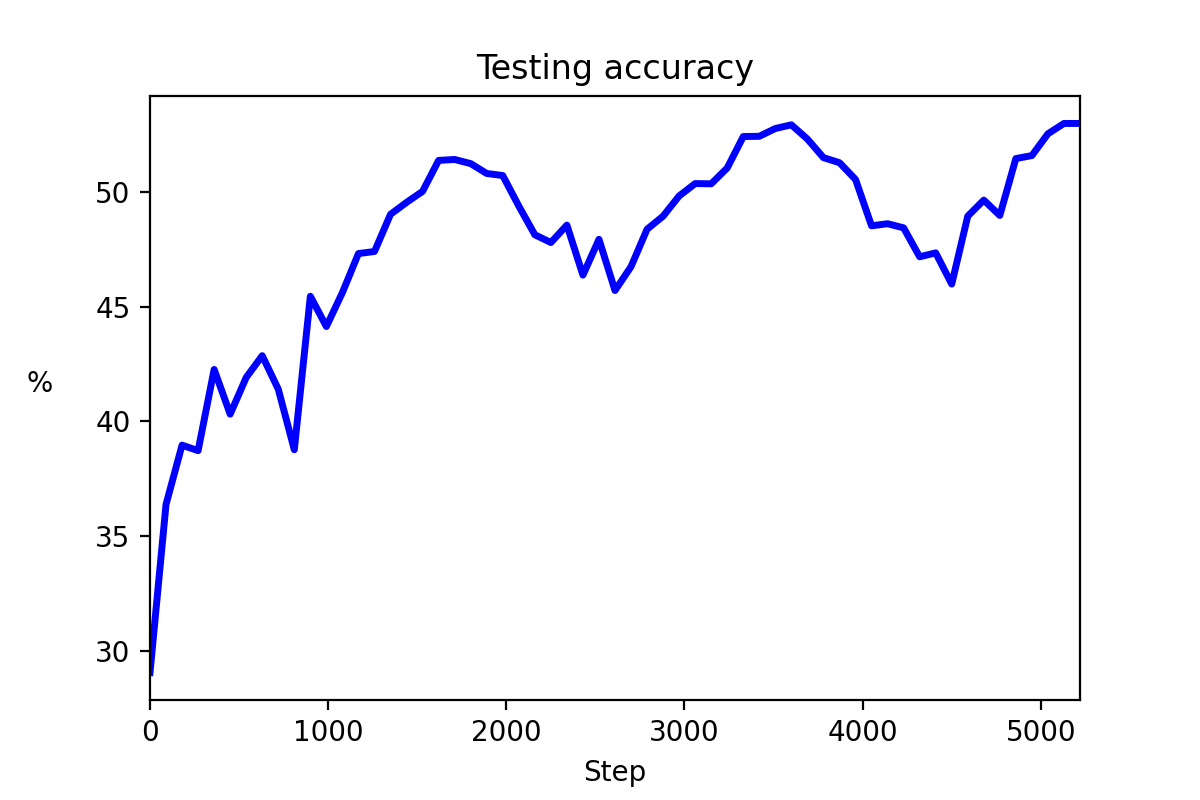
\includegraphics[width=6cm]{../plots/cyclical/acc_v0.png}
%		\vspace{0.1cm}
%		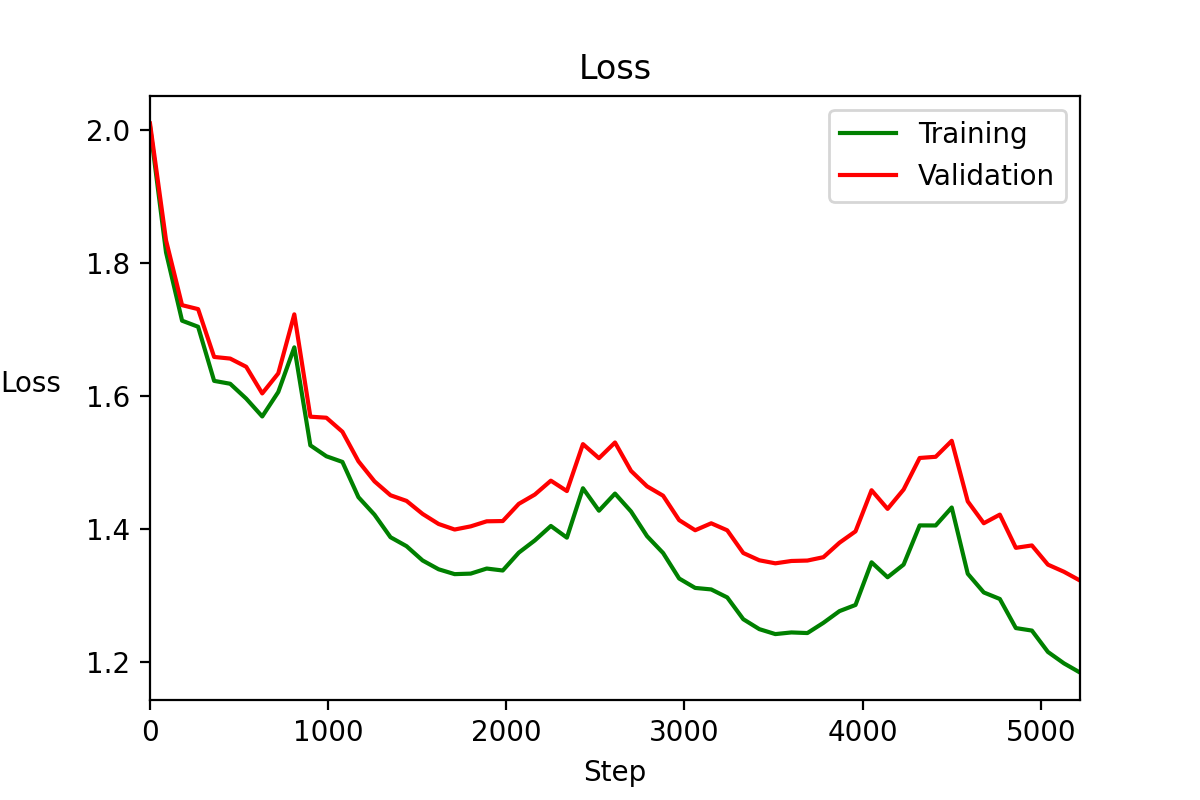
\includegraphics[width=6cm]{../plots/cyclical/loss_v1.png}
%		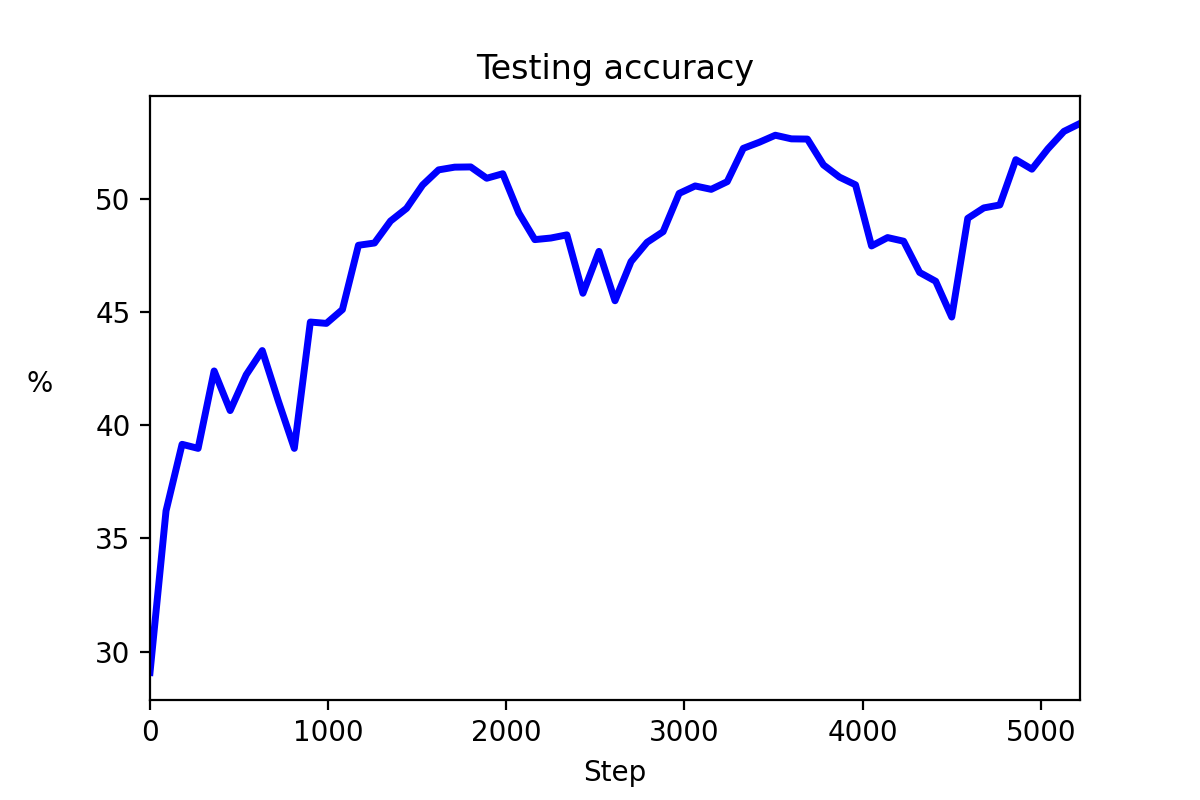
\includegraphics[width=6cm]{../plots/cyclical/acc_v1.png}
%		\vspace{0.1cm}
%		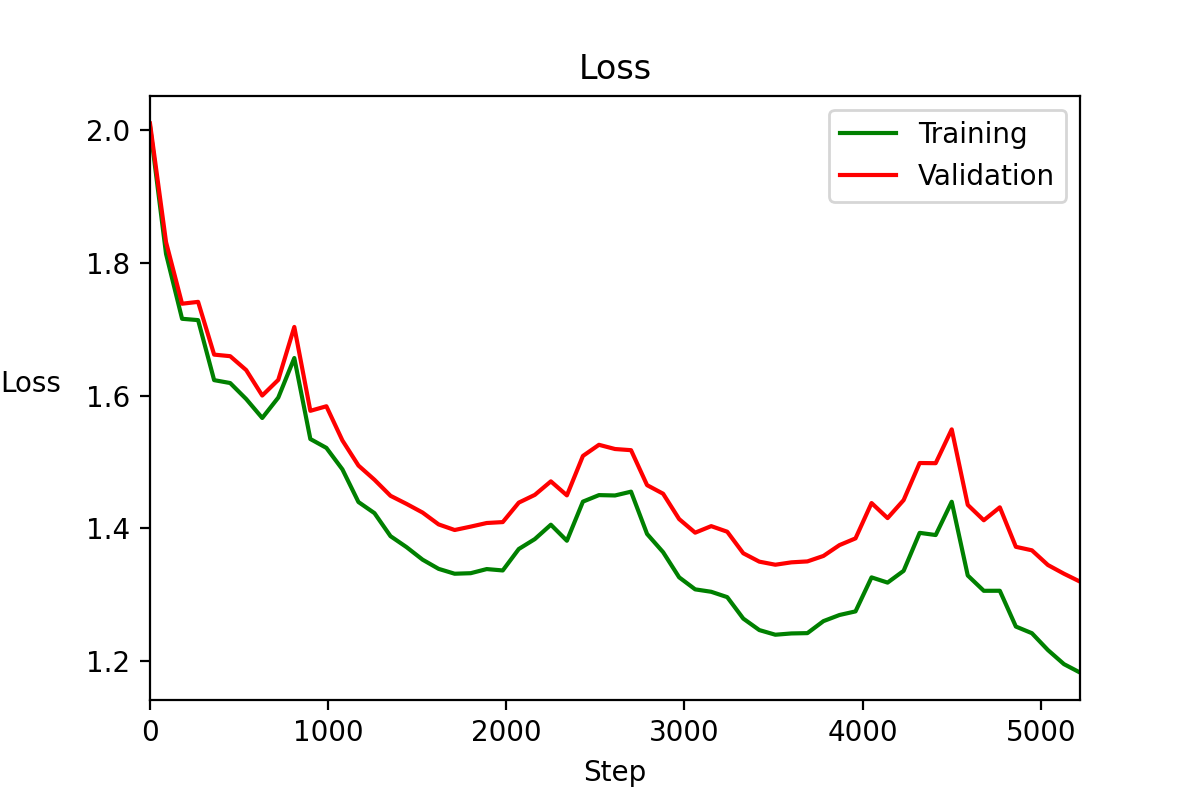
\includegraphics[width=6cm]{../plots/cyclical/loss_v2.png}
%		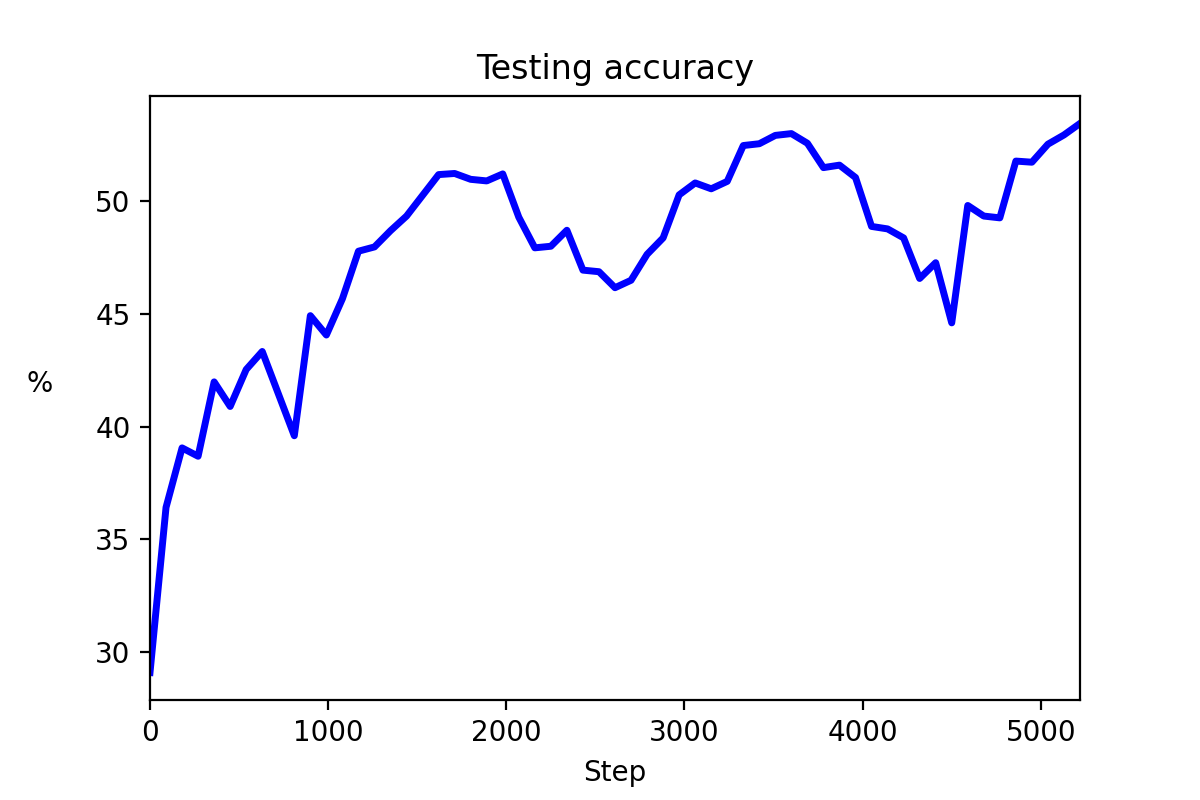
\includegraphics[width=6cm]{../plots/cyclical/acc_v2.png}
%		\vspace{0.1cm}
%		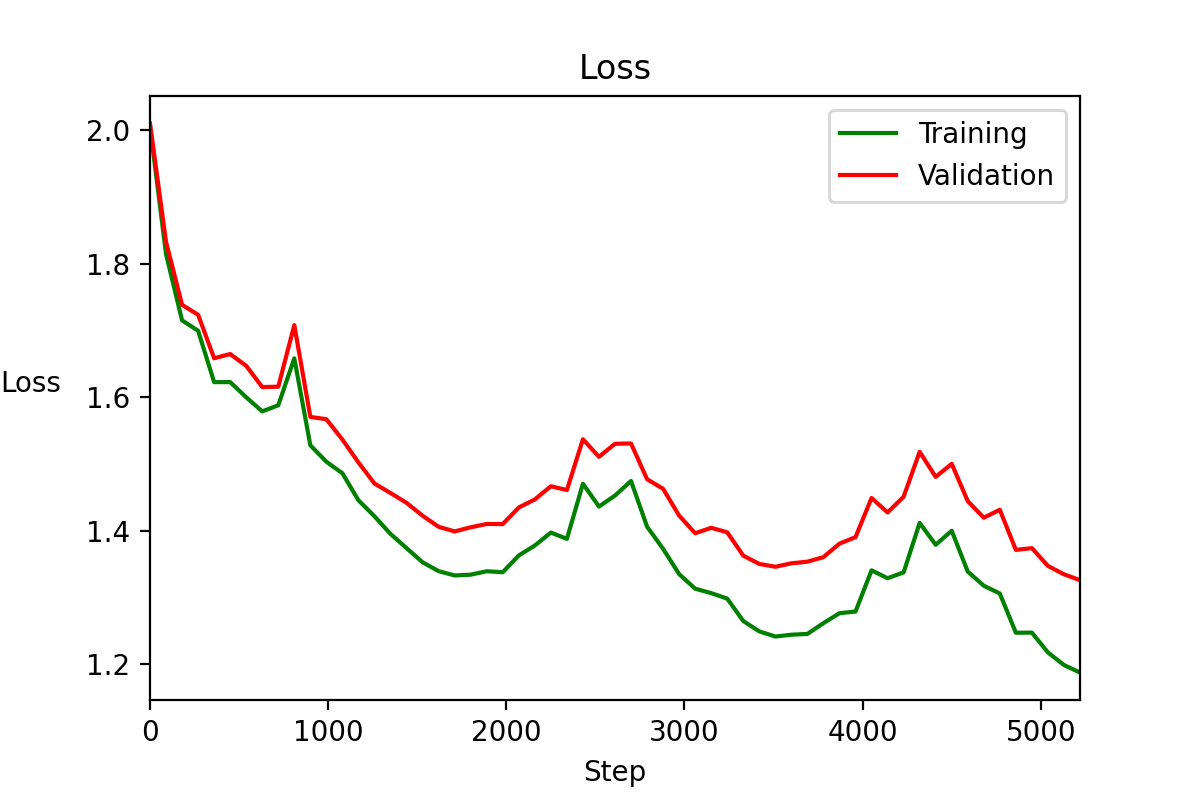
\includegraphics[width=6cm]{../plots/cyclical/loss_v3.png}
%		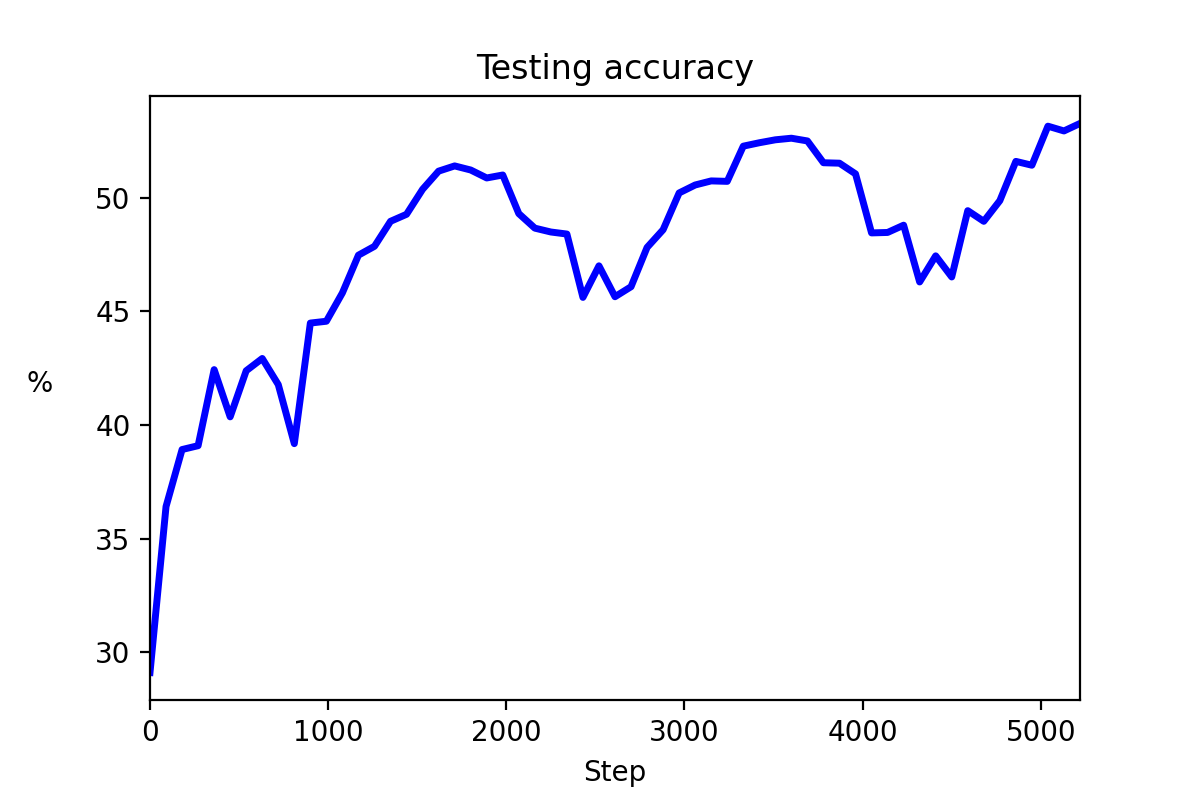
\includegraphics[width=6cm]{../plots/cyclical/acc_v3.png}
%		\vspace{0.1cm}
%		\caption{Loss and testing accuracy when using $m=100$ with a $0.2$ dropout rate, image flipping, image translations and a cyclical learning rate - for $\lambda\in\{0.0001, 0.0002, 0.00025, 0.0003\}$}
%	\end{figure}

\newpage
\subsection*{Using Momentum}
	To further try and squeeze out some marginal gains on the training accuracy, I implemented a different scheme for the gradient updates and learning rate. While the Nesterov Accelerated Gradient was suggested, I was interested in how the very popular Adam optimizer works. Hence, I implemented the Adam optimizer for the $2$-layer neural network, using the standard parameter settings, i.e. 
	\begin{itemize}
		\item $\beta_1 = 0.9$,
		\item $\beta_2 = 0.999$,
		\item $\eta = 0.01$,
		\item $\epsilon = 10^{-8}$
	\end{itemize}
	In order to compare the effect of employing the Adam oprimizer with that of the previous scheme, I trained the network for the same number of steps, i.e. corresponding to $3$ cycles with \texttt{nt}$=450$. I also used the same probabilities for augmenting the data, i.e. an image was flipped with $p_{flip} = 0.2$ and translated with $p_{translate} = 0.05$. Again, there were $100$ hidden nodes, combined with a dropout rate of $0.2$. The results for the same set of $\lambda$ values are symmarized in the table below, along with loss and accuracy plots for the top-performing parameter settings. Overall, the performance is very similar - in fact the cyclical learning rate with a normal SGD update seems to outperform the Adam optimizer to some degree. However, the latter is clearly more stable and converges to a solution without the cyclical components in the loss and accuracy seen when using the cyclical learning rate. 
	\vspace{0.3cm}
	\begin{center}	
	\begin{tabular}{|l|c|}
		\hline
		 $\lambda$ & \text{Accuracy}, \% \\ \hline
		0.0001 & 52.63\\ 
		0.0002 & 52.07\\
		0.00025 & 52.09\\
		0.0003 & 51.80\\\hline
	\end{tabular}
	\end{center}

	\begin{figure}[!h]
	\centering
	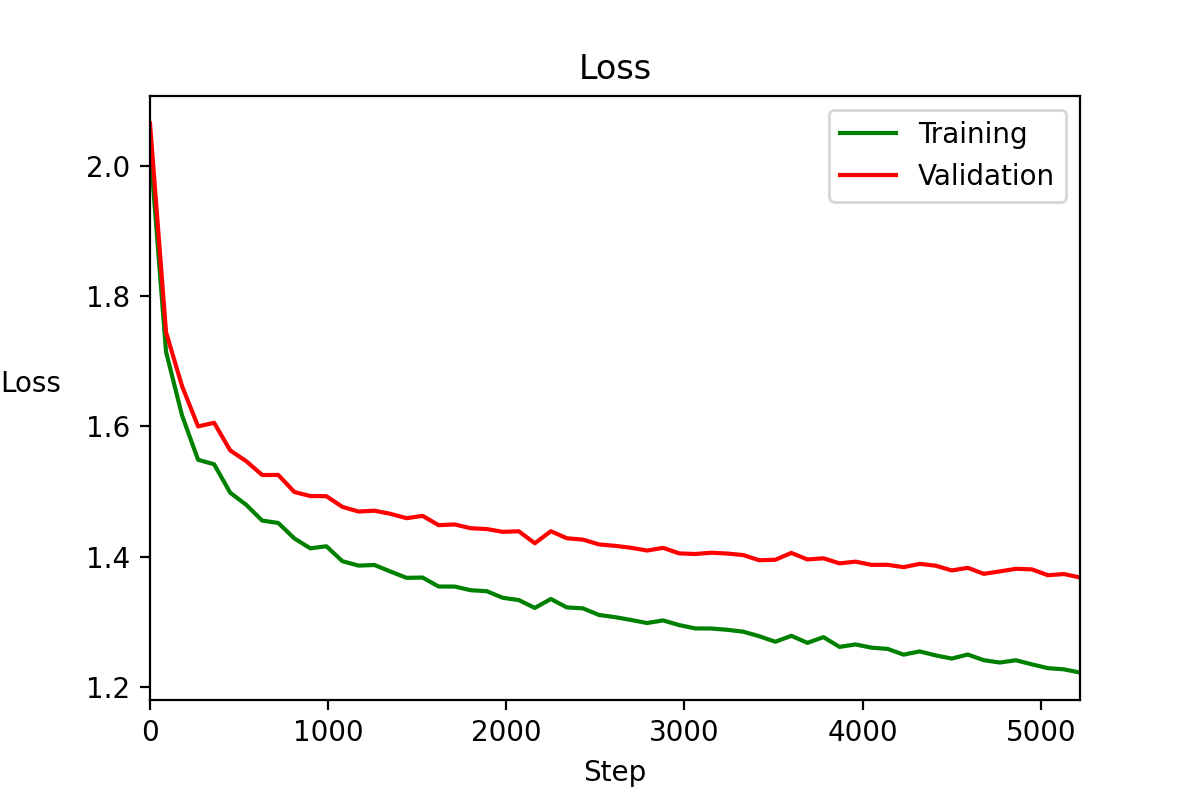
\includegraphics[width=6cm]{../plots/adam/loss_v0.png}
	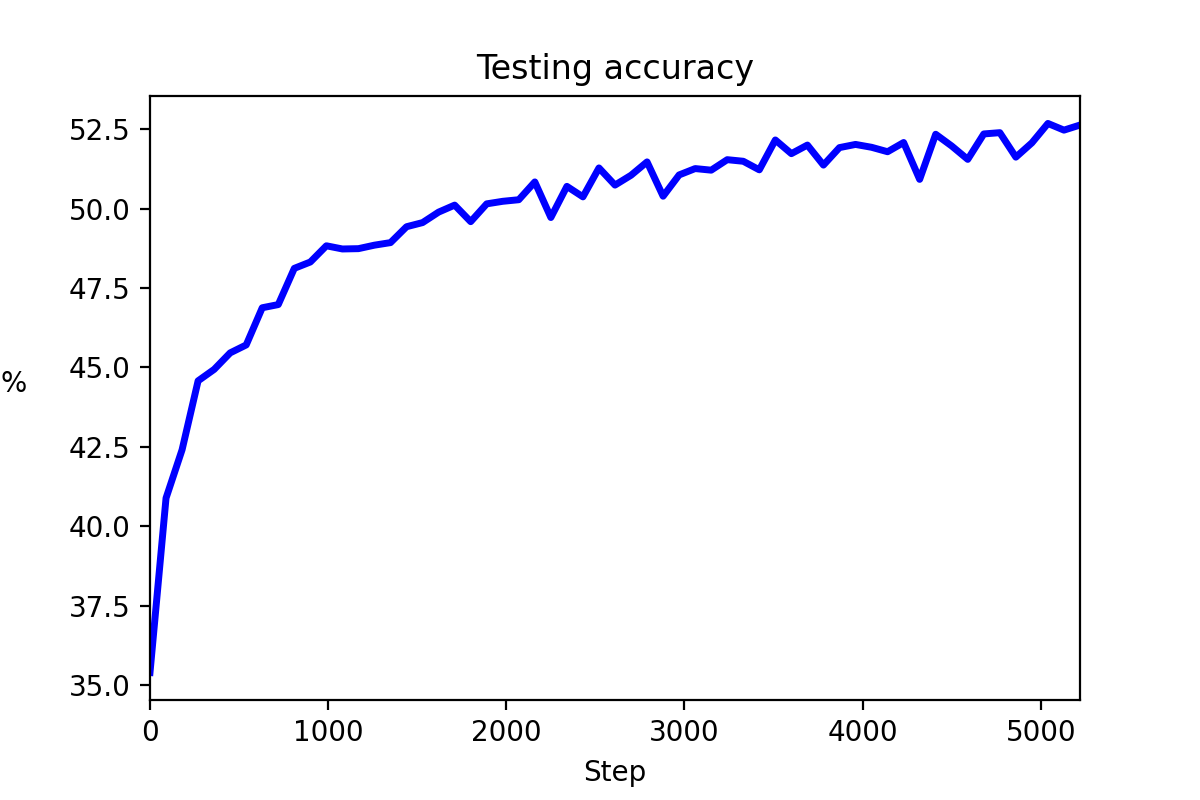
\includegraphics[width=6cm]{../plots/adam/acc_v0.png}
	\caption{Loss and testing accuracy when using $m=100$ with a $0.2$ dropout rate, image flipping, image translations and a cyclical learning rate - using an Adam optimizer and $\lambda = 0.0001$.}
	\end{figure}

\newpage

\section*{Part II}
	For this part, I changed the data-augmentation parameters slightly. Instead of using $p_{flip} = 0.2$, the data-augmentation used $p_{flip} = 0.4$ with the same probability for translation, i.e. $p_{translate} = 0.05$. For each parameter setting, training was run for a number of steps corresponding to $2$ cycles with \texttt{nt}$=450$. The parameters tested were the following:
	\begin{itemize}
		\item $\lambda \in \{5\cdot10^{-5}, 10^{-4}\}$, 
		\item $m \in \{50, 75, 100, 125, 150\}$,
		\item $p_{drop} \in \{0.0, 0.2, 0.3, 0.4, 0.5\}$
	\end{itemize}
	\vspace{0.2cm}
	The full results are summarized in the table on the last page, and the effects across different settings are illustrated in the histograms in Figure $3$. Overall, the results are somewhat similar to those obtained previously, i.e. an accuracy in the $50-53$\% range. However, there seem to be some trends across the $50$-something testing results: \textit{larger networks} with \textit{low or no dropout} achieves the best performance.\\
	\begin{figure}[!h]
		\centering
		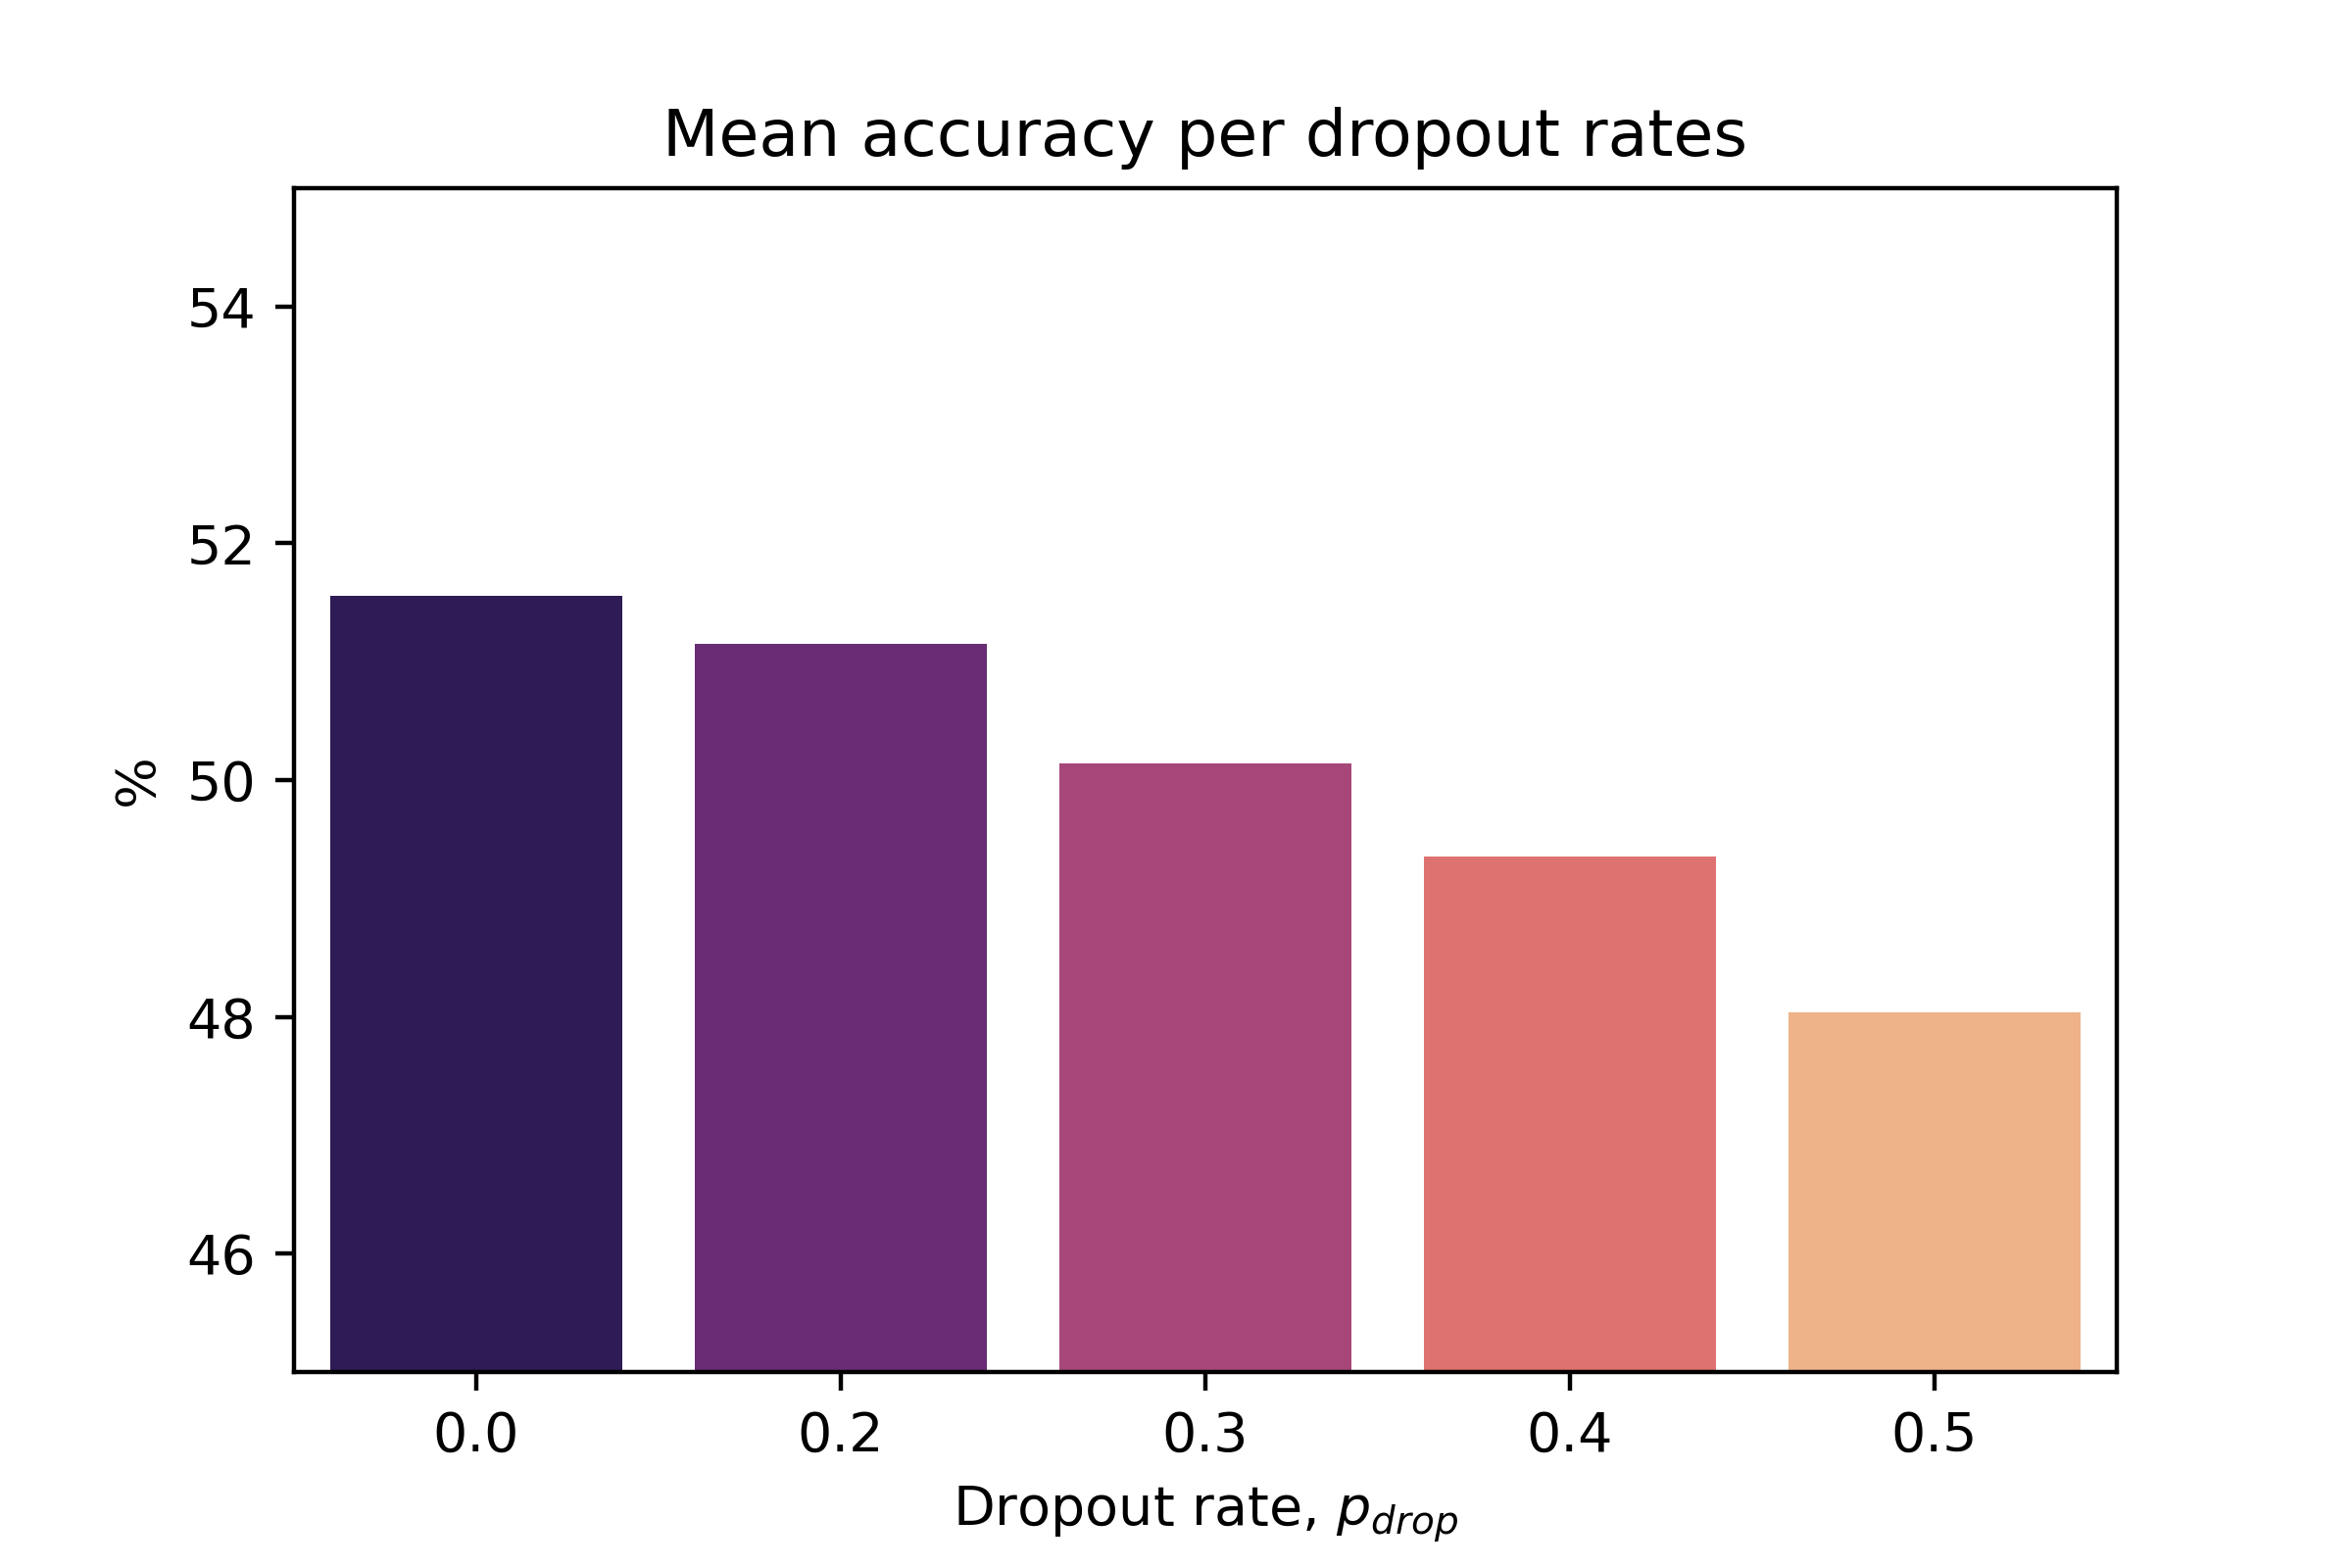
\includegraphics[width=6cm]{../plots/compDropout.png}
		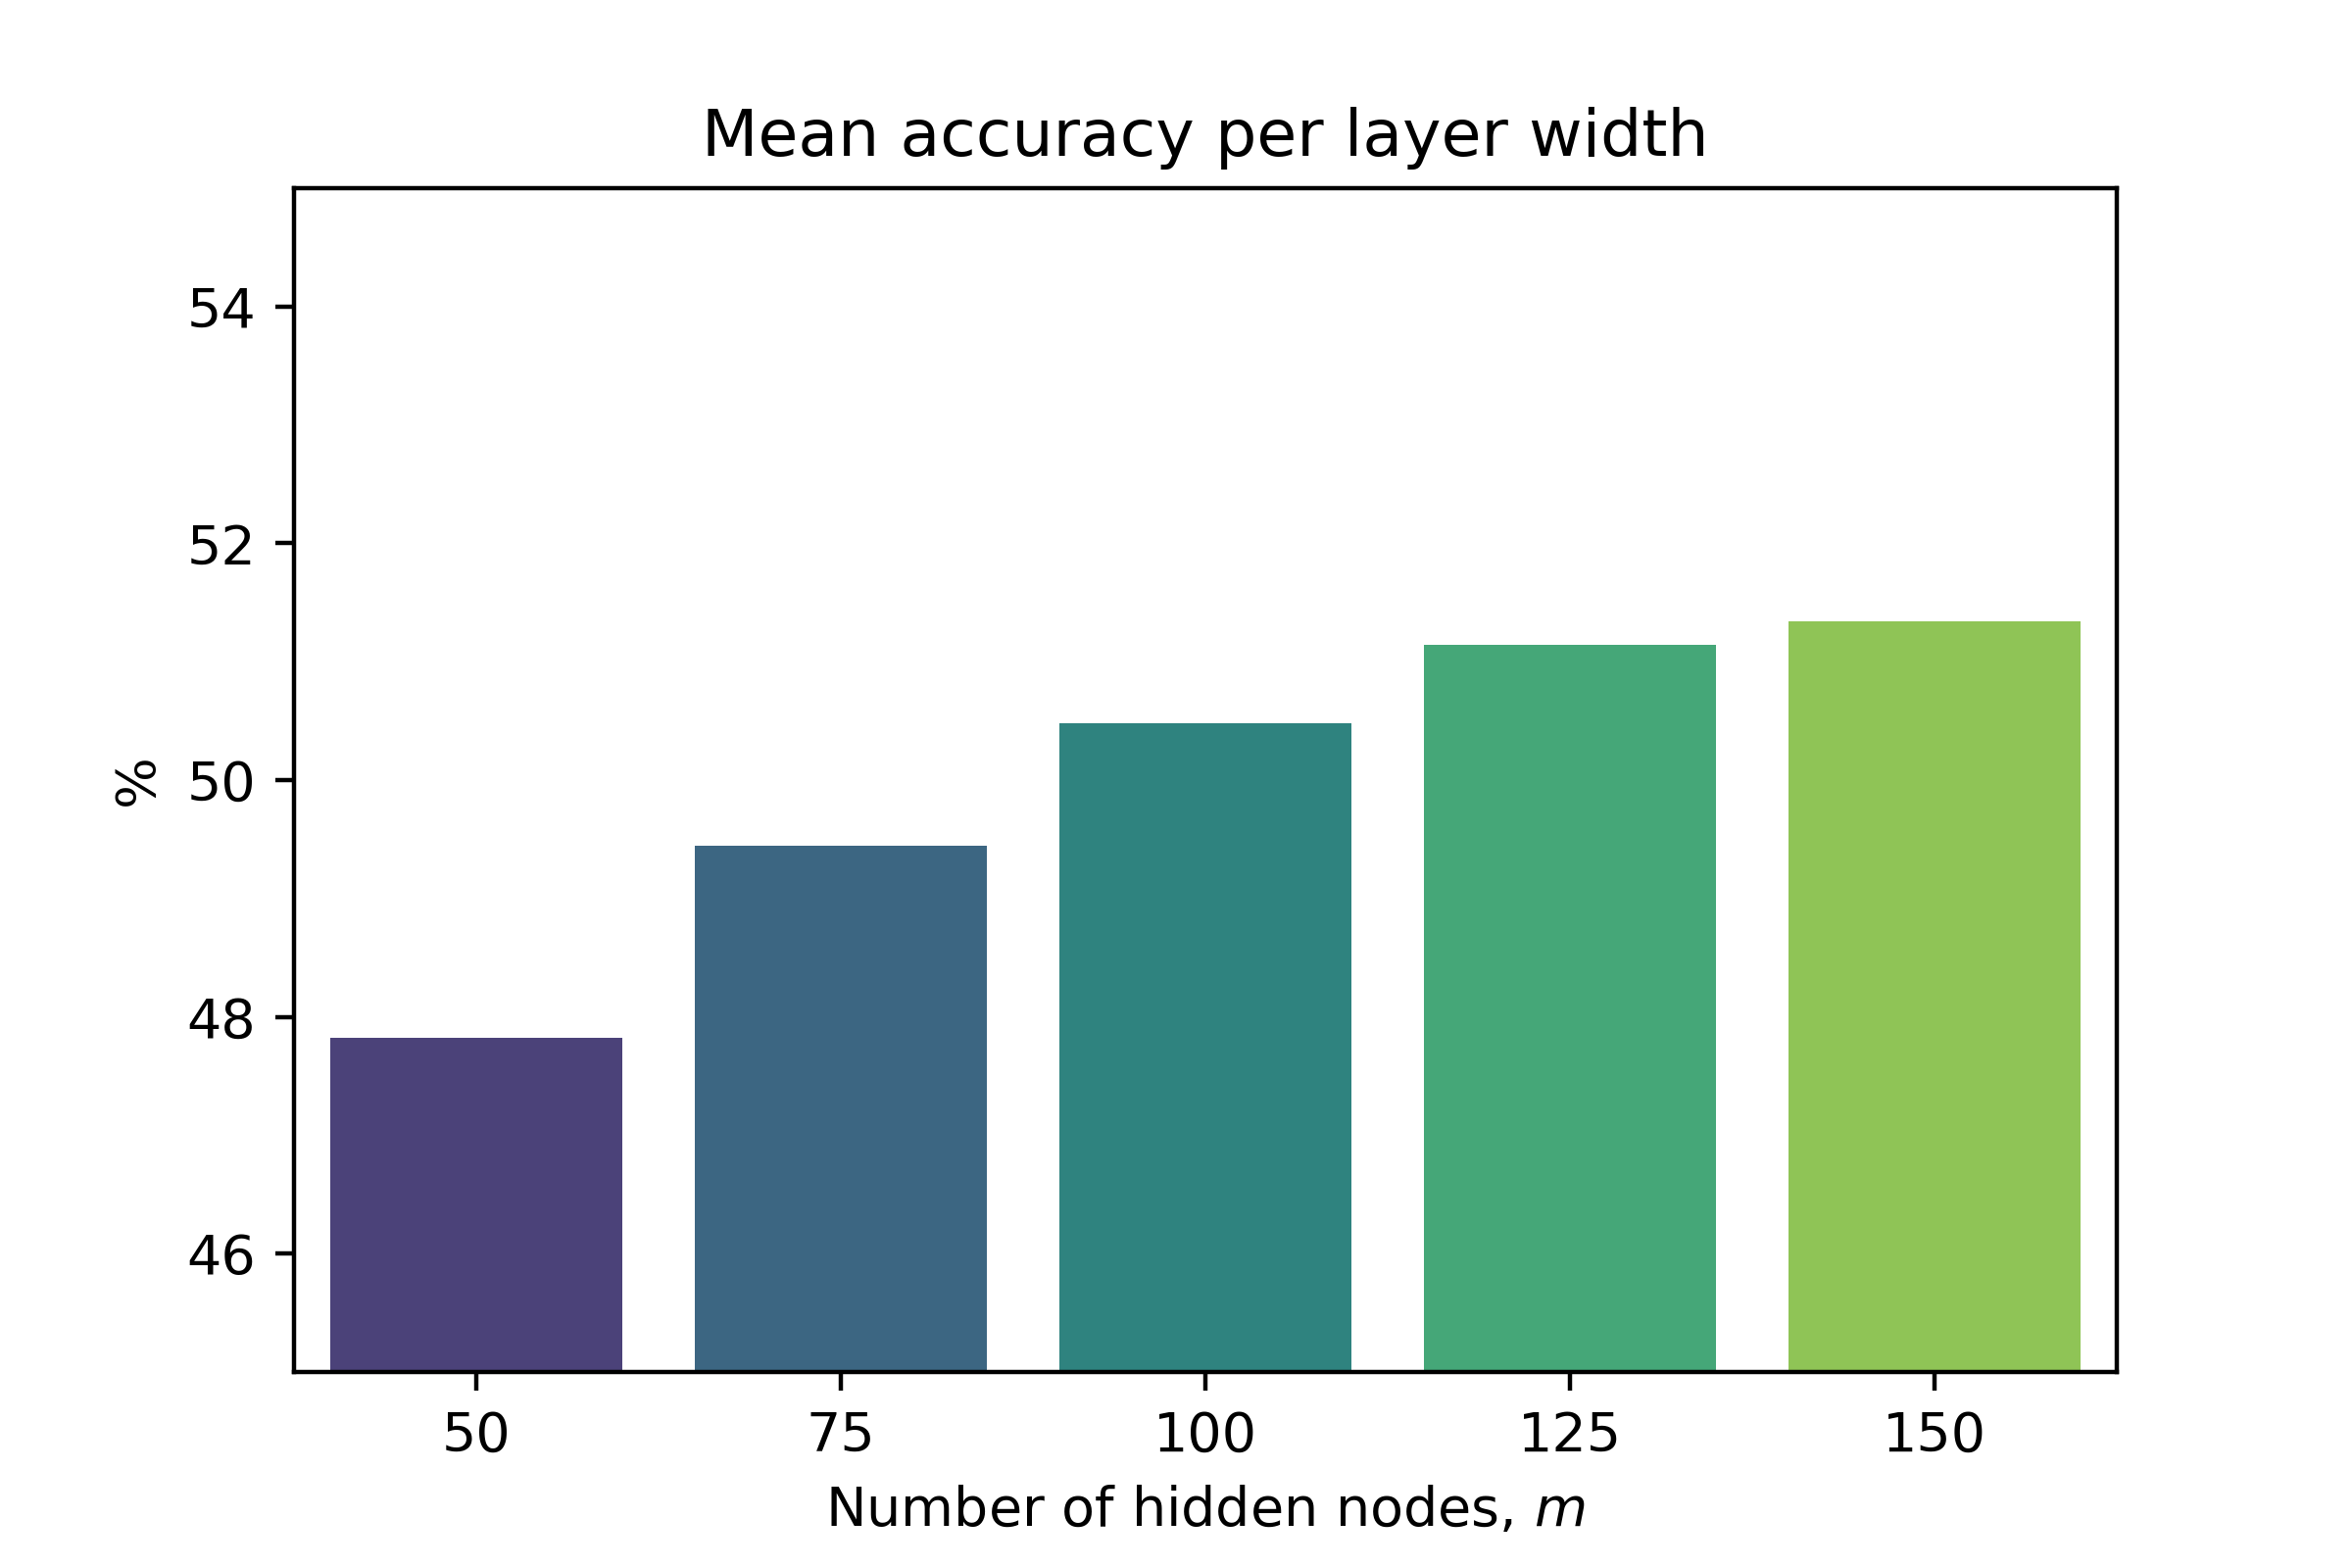
\includegraphics[width=6cm]{../plots/compLayerM.png}
		\caption{Mean testing accuracy for varying layer width, $m$, and dropout rate, $p_{drop}$.}
	\end{figure}\\
	It seems that there is a clearly positive effect on the testing accuracy when employing a wider network. However, the marginal gain does seem to be decreasing and it is not clear that it is possible to achieve a much higher accuracy than $55-56$\% with more hidden nodes. Rather, we likely have to employ more hidden layers and more regularization. But in the case of a $2$-layer neural network, it seems the most significant improvements are data augmentation (especially horizontal image flipping) and more hidden nodes, with improvements up to $m \leq 300$. Following this result, I trained a number of wide networks with no dropout and for varying $\lambda$ values and for longer training periods. When abandoning the cyclical learning rate and using e.g. an Adam optimizer, the network benefits from a longer training period. The results for the wider networks trained on a longer period are summarized below:
	\vspace{0.3cm}
	\begin{center}	
		\begin{tabular}{|l|l|l|c|}
			\hline
			 $\lambda$ & $m$ & $p_{drop}$ & Accuracy, \% \\\hline
			0.00005 & 200 & 0.0 & 55.54 \\
			0.0001 & 200 & 0.0 & 55.90 \\
			0.0002 & 200 & 0.0 & 55.32 \\
			0.0002 & 150 & 0.0 & 54.52 \\
			0.001 & 150 & 0.0 & 54.58 \\\hline
		\end{tabular}
	\end{center}


\newpage
\subsection*{Final results}
	I trained larger networks with $m\in\{150, 200\}$ and $p_{drop} = 0.0$ with different $\lambda$ values for longer training periods and eventually achieved an accuracy of $\bm{55.9}$\%. The performance of the best network is illustrated in Figure $4$ below. It seems unlikely that an even wider network would be able to squeeze out much more in the margins. However, there might be some other combination of data augmentation and regularization that could perform even better, perhaps more translations and more dropout. However, from some preliminary testing this does not seem to be the case. Rather, the network seems to benefit form a low $\lambda$ and a low or no dropout rate, while the most significant improvements seem to depend on data augmentation and the size of the network - as well as prolonging the training period when using momentum rather than a cyclical learning rate.
	\begin{figure}[!h]
		\centering
		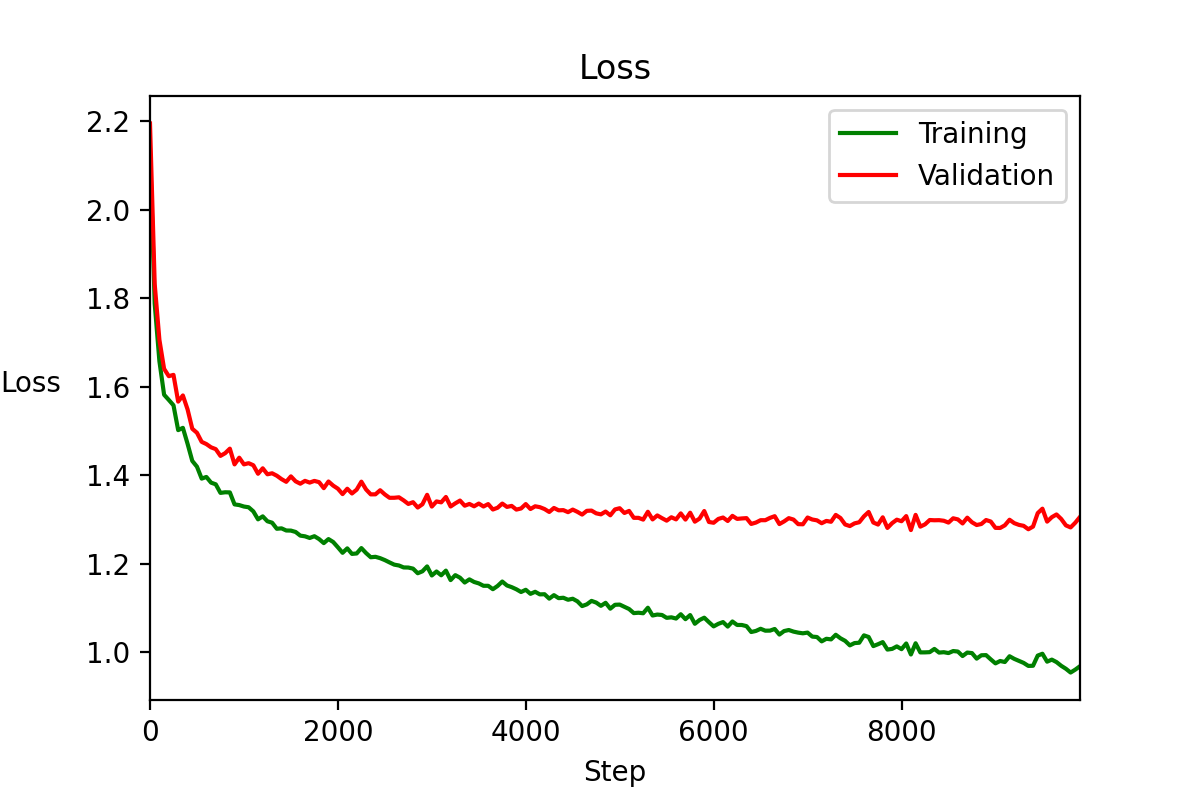
\includegraphics[width=9cm]{../plots/loss_top_v3.png}
		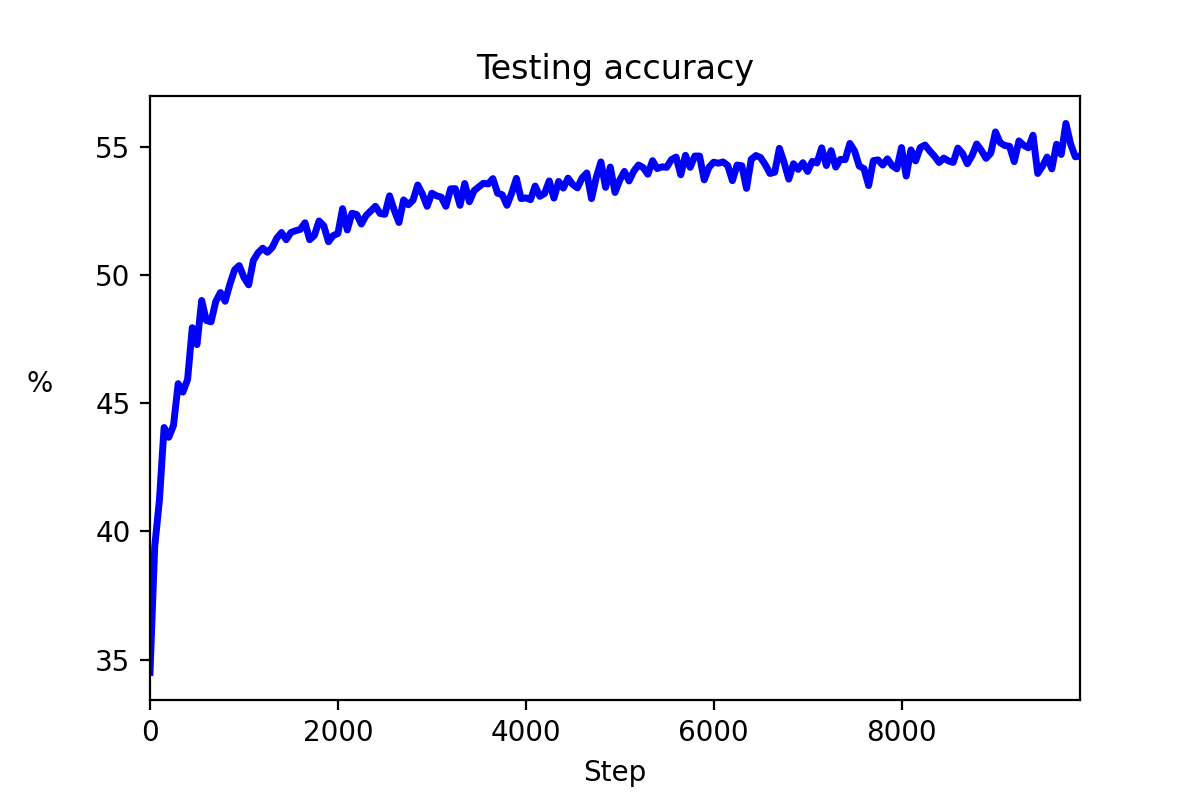
\includegraphics[width=9cm]{../plots/acc_top_v3.png}
		\caption{Loss and testing accuracy for a $2$-layer network with an Adam optimizer and $m = 200$, $p_{drop} = 0.0$, $\lambda = 5\cdot10^{-5}$, $p_{flip}=0.4$, $p_{transl}=0.05$.}
	\end{figure}
	

\newpage
	\begin{center}	
	\begin{tabular}{|l|l|l|c|}
		\hline
		 $\lambda$ & $m$ & $p_{drop}$ & Accuracy, \% \\\hline
		0.00005 & 50 & 0.20 & 49.0500 \\
		0.00005 & 50 & 0.30 & 48.1200 \\
		0.00005 & 50 & 0.40 & 46.8200 \\
		0.00005 & 50 & 0.50 & 45.3800 \\
		0.00005 & 75 & 0.20 & 50.8600 \\
		0.00005 & 75 & 0.30 & 49.3700 \\
		0.00005 & 75 & 0.40 & 48.5000 \\
		0.00005 & 75 & 0.50 & 47.4800 \\
		0.00005 & 100 & 0.20 & 51.4700 \\
		0.00005 & 100 & 0.30 & 50.2100 \\
		0.00005 & 100 & 0.40 & 49.8000 \\
		0.00005 & 100 & 0.50 & 48.6400 \\
		0.00005 & 125 & 0.20 & 52.1000 \\
		0.00005 & 125 & 0.30 & 51.3400 \\
		0.00005 & 125 & 0.40 & 50.3500 \\
		0.00005 & 125 & 0.50 & 49.2500 \\
		0.00010 & 50 & 0.20 & 48.8900 \\
		0.00010 & 50 & 0.30 & 48.1700 \\
		0.00010 & 50 & 0.40 & 47.1500 \\
		0.00010 & 50 & 0.50 & 45.6200 \\
		0.00010 & 75 & 0.20 & 50.7500 \\
		0.00010 & 75 & 0.30 & 49.6000 \\
		0.00010 & 75 & 0.40 & 48.6200 \\
		0.00010 & 75 & 0.50 & 46.9700 \\
		0.00010 & 100 & 0.20 & 51.9500 \\
		0.00010 & 100 & 0.30 & 50.2600 \\
		0.00010 & 100 & 0.40 & 49.9100 \\
		0.00010 & 100 & 0.50 & 48.6800 \\
		0.00010 & 125 & 0.20 & 52.0700 \\
		0.00010 & 125 & 0.30 & 51.5300 \\
		0.00010 & 125 & 0.40 & 50.6600 \\
		0.00010 & 125 & 0.50 & 49.5500 \\
		0.00005 & 50 & 0.00 & 49.4600 \\
		0.00005 & 75 & 0.00 & 51.0000 \\
		0.00005 & 100 & 0.00 & 51.9900 \\
		0.00005 & 125 & 0.00 & 52.3700 \\
		0.00010 & 50 & 0.00 & 49.5400 \\
		0.00010 & 75 & 0.00 & 51.3100 \\
		0.00010 & 100 & 0.00 & 51.9100 \\
		0.00010 & 125 & 0.00 & 52.2400 \\
		0.00005 & 150 & 0.20 & 52.1500 \\
		0.00005 & 150 & 0.30 & 51.4600 \\
		0.00005 & 150 & 0.40 & 50.8500 \\
		0.00005 & 150 & 0.50 & 49.5100 \\
		0.00005 & 150 & 0.00 & 53.0100 \\
		0.00010 & 150 & 0.20 & 52.2100 \\
		0.00010 & 150 & 0.30 & 51.3100 \\
		0.00010 & 150 & 0.40 & 50.8500 \\
		0.00010 & 150 & 0.50 & 49.3000 \\
		0.00010 & 150 & 0.00 & 52.7700 \\\hline
	\end{tabular}
	\end{center}



\end{document}